\chapter{Related Works}
\label{chap:related_works}

\section{Speech Synthesis}
\label{sec:speech_synthesis}
Initially, TTS research focused on combining acoustic models, which convert text into audio spectrograms, with vocoders that synthesize these spectrograms into audible speech.
These early systems\cite{Fastspeech2}, while groundbreaking, often produced speech that lacked naturalness and was easily distinguishable from human speech.
Despite advancements, traditional TTS systems faced notable challenges. One significant issue was their performance in noisy environments, where the quality and intelligibility of synthesized speech often degraded.
Additionally, the language-specific nature of these systems meant that introducing a new language required extensive data collection and model retraining, a process that was resource-intensive and limited the scalability of TTS technology, especially for languages with fewer resources.
In response to these challenges, recent research\cite{Vall-E-X}, discribed in \ref{fig:Valle} has shifted towards neural audio codec-based TTS. This approach leverages advanced neural network architectures to improve the robustness, naturalness, and expressiveness of synthesized speech.
Neural audio codecs have shown a remarkable ability to maintain speech clarity in noisy environments, a significant improvement over traditional methods.
Furthermore, neural audio codecs are language-agnostic, meaning that they can be trained on a single dataset and used to synthesize speech in any language, thereby eliminating the need for language-specific models and data collection.

\begin{table}[h]
    \begin{center}
    % \small
    \caption{A comparison between neural audio codec based TTS and previous TTS systems.}
    \label{table_compare}
    \begin{tabular}{c|c|c}
    \toprule
    & \bf Previous Systems  & \textbf{Vall-E-X} \\  \hline
    Intermediate representation & Mel spectrogram   &   Audio codec codes \\ \hline
    Training data & $<$ 13K hours   & 70K hours   \\ \hline
    Speech accent &  Foreign    &  Native  \\  \hline
    Speaker similarity & Relative low   &  High  \\  \hline
    In-context learning & \xmark   & \cmark  \\ \hline
    Zero-shot cross-lingual TTS & \xmark   & \cmark  \\ 
    \bottomrule
    \end{tabular}
    \label{adv}
    \end{center}
\end{table}
    
\subsection{Neural Audio Codec based TTS}
\label{subsec:neural_audio_codec_based_tts}
\begin{figure}
    \centering
    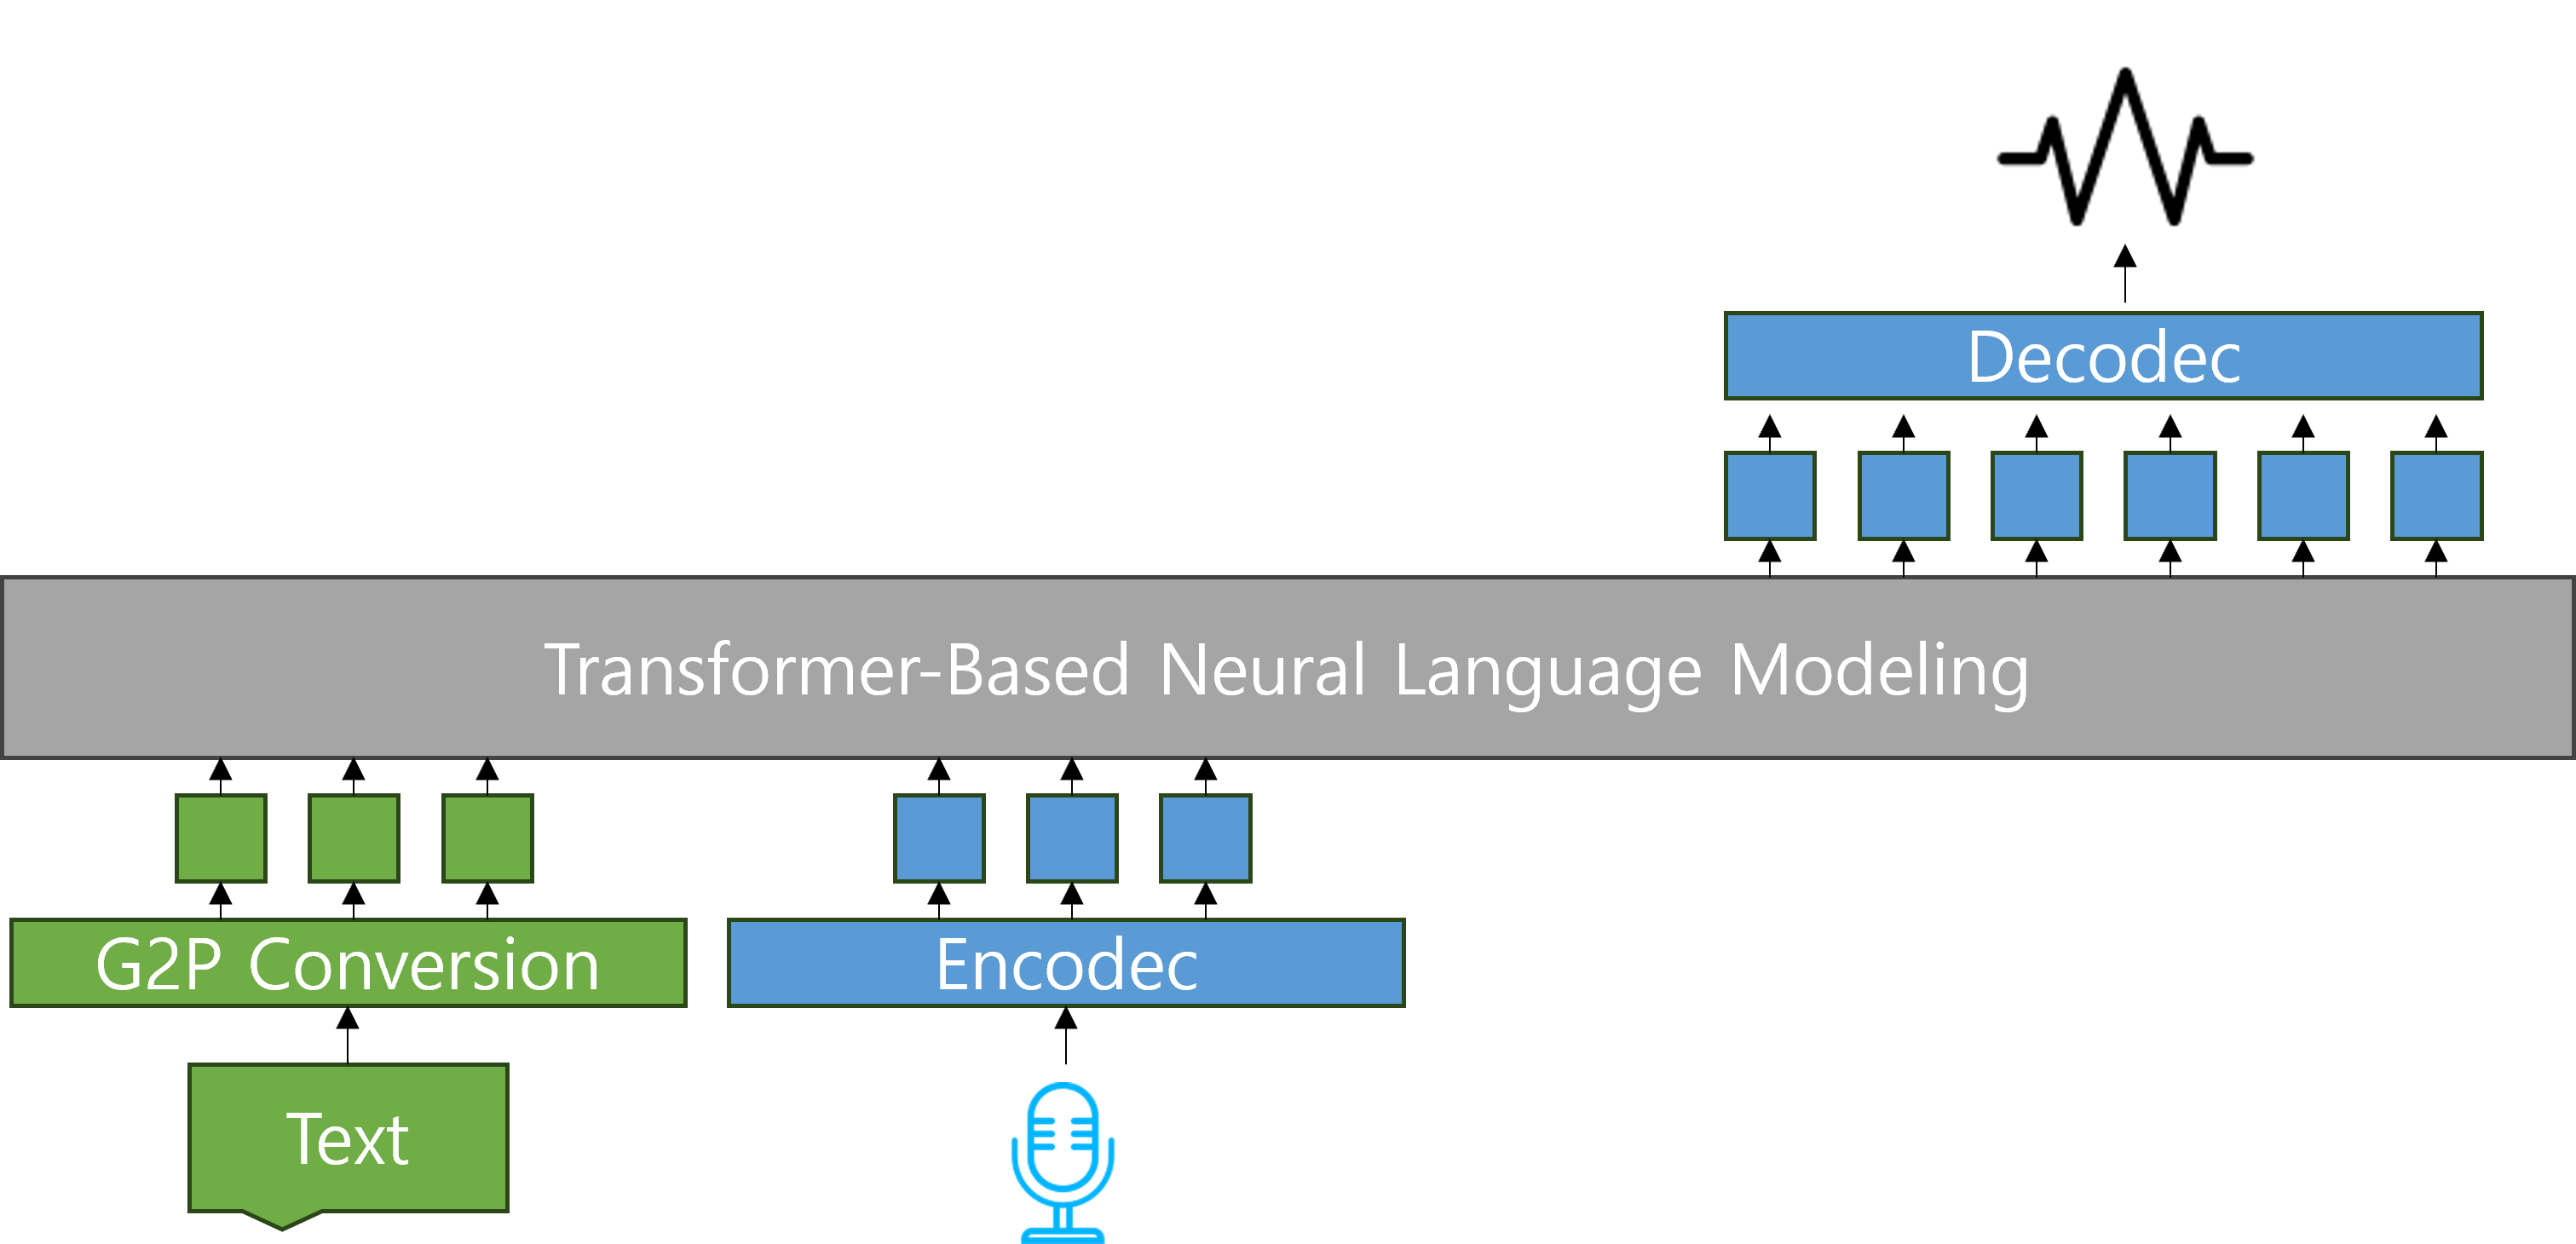
\includegraphics[width=0.8\textwidth]{figures/figure_chap_2/valle.png}
    \caption{Neural Audio Codec based TTS}
    \label{fig:Valle}
\end{figure}
Neural audio codec based TTS is an method regarding TTS as conditional codec language modeling.
Vall-E-X\cite{Vall-E-X} is a notable method. It consists of three modules, phoneme embedding and audio-to-codec module, trasformer-based codec-to-codec module, and a codec-to-audio module.
The dataset consists of pairs ${\mathbf{x}_i , \mathbf{y}_i }$, where $\mathbf{y}_i$ is an audio sample and $\mathbf{x}_i$ is the corresponding phoneme transcription.
The phoneme embedding and audio-to-codec module is trained to encode audio prompt and text prompt.
Each audio sample $\mathbf{y}$ is encoded into discrete acoustic codes using a pre-trained neural codec model\cite{EnCodec}, denoted as $\text{Encodec}(\mathbf{y}) = \mathbf{C}^{T \times 8}$. Here, $\mathbf{C}$ is a two-dimensional acoustic code matrix.
The row vector $\mathbf{c}_{t,:}$ represents the eight codes for frame $t$. Each frame captures a segment of the audio at a specific time.
The column vector $\mathbf{c}_{:, j}$ represents the code sequence from the $j$-th codebook. The codebooks can be thought of as libraries of distinct sound units, where $j \in {1, \ldots, 8}$.

\begin{figure}
    \centering
    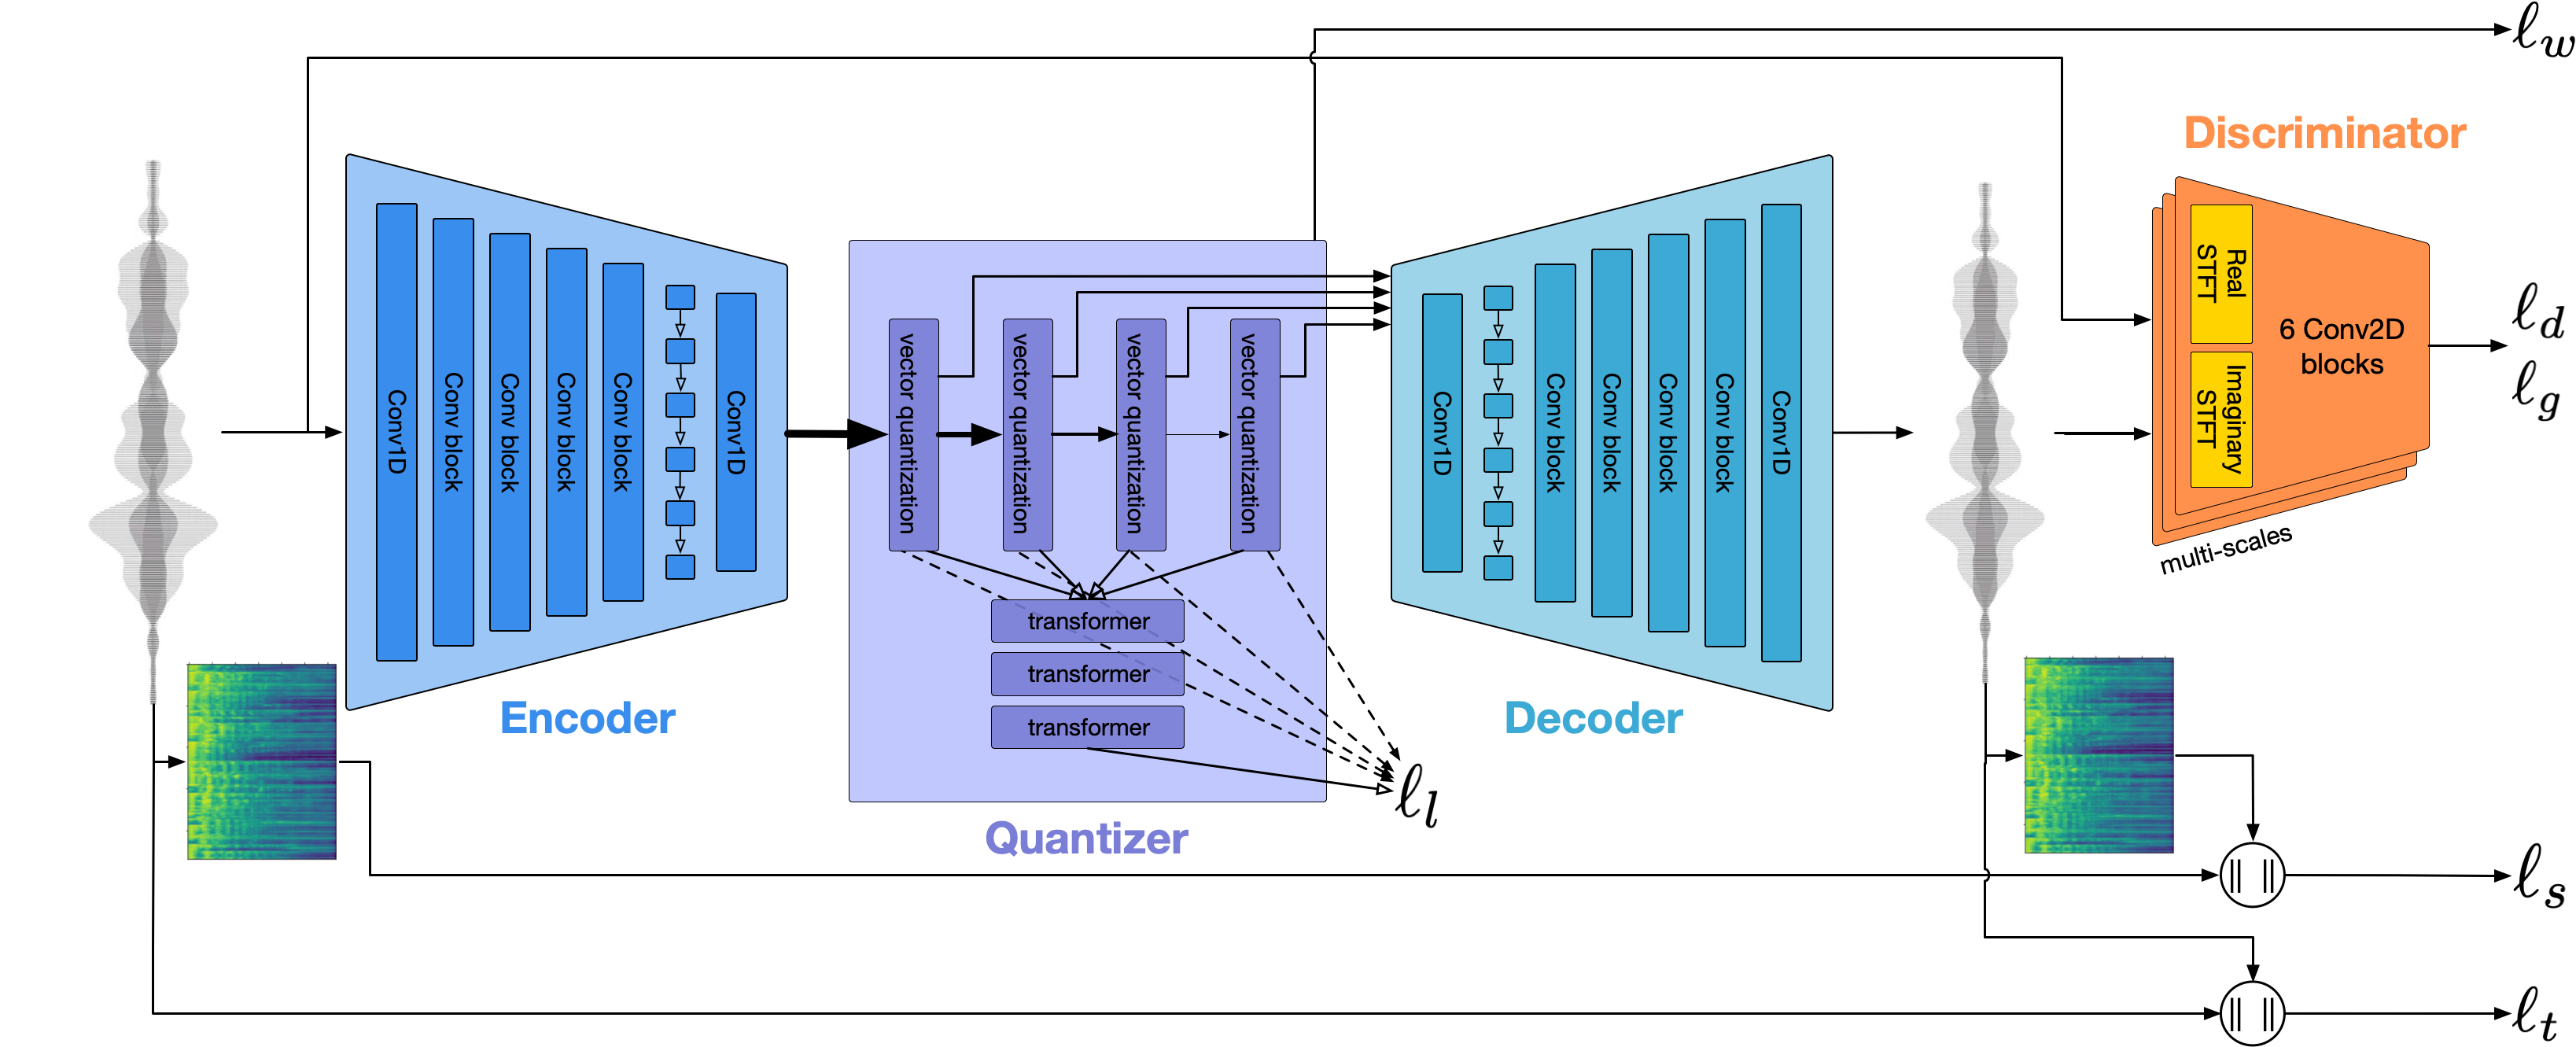
\includegraphics[width=0.8\textwidth]{figures/figure_chap_2/encodec.png}
    \caption{pre-trained neural codec model Architecture}
    \label{fig:EnCodec}
\end{figure}

The transformer-based codec-to-codec module is trained to combine acoustic and linguistic information.
To balance the trade-off between audio quality and inference speed, this module combine AR and NAR, decoder-only models.
The AR model is conditioned on the phoneme sequence $\mathbf{x}$ and the first column of the acoustic code matrix, $\mathbf{{C}}_{:,1}$. 
\begin{equation}
\label{AR}
    p (\mathbf{c}_{:,1} | \mathbf{x}, \mathbf{\tilde{C}}_{:,1}; \theta_{AR}) = \prod_{t=0}^{T} p(\mathbf{c}_{t, 1}|\mathbf{ c}_{<t, 1}, \mathbf{\tilde{c}}_{:,1}, \mathbf{x}; \theta_{AR})
\end{equation} 
The NAR model has similar architecture to the AR model, but it is conditioned on the entire acoustic code matrix $\mathbf{\tilde{C}}$.
\begin{align}
    e_{c_{t,j}} &= W_a^j \odot {c_{t,j}} \\
    \mathbf{e_{c_t}} &= \sum_{j=1}^{i-1} e_{c_t,j}
\end{align}
The reason for dividing the tokens referenced by the Autoregressive (AR) and Non-Autoregressive (NAR) models in this way lies in the nature of the information encoded in the residual tokens. Encodec \cite{EnCodec} encodes audio using residual vector quntization, the first residual token in the input sequence is particularly dominant in terms of the information it contains. Therefore, the AR model is conditioned on the first residual token, while the NAR model is conditioned on the entire residual token sequence.
The codec-to-audio module is trained to decode the acoustic codes into audio samples. The model discribed at decoder part of \ref{fig:EnCodec}.

\section{Talking Head Generation}
\label{sec:talking_head_generation}

\subsection{Text-Driven}
\label{subsec:text_driven}
Text-driven talking head generation is a task that generates a video of a person speaking a given text.
Text2Video\cite{Text2Video} is a notable method. It starts by converting text to speech, followed by aligning the generated audio with the text using the Montreal Text Aligner.
This alignment informs the smoothing of a phoneme-pose dictionary, leading to the creation of a face landmark array. The final video is generated using Generative Adversarial Networks (GANs), which transform the face landmark array into realistic images.
However, a key limitation of Text2Video is the potential lack of naturalness in the transition of generated frames, as the reliance on GANs can sometimes result in less fluid and lifelike facial movements.

\subsection{Audio-Driven}
\label{subsec:audio_driven}
Audio-driven talking portrait synthesis is designed to animate a specific individual's portrait using given speech audio. Various techniques have been developed to create realistic and synchronized talking portrait videos.
Early methods relied on predefined rules linking phonemes to mouth movements, using stitching techniques to modify mouth shapes.

The introduction of deep learning led to the development of image-based methods, which synthesize images directly from audio inputs.
These methods, however, are generally limited to producing images at a fixed resolution and do not offer control over head poses.

Another approach involves model-based methods, which utilize structural representations like facial landmarks and 3D face models to aid in the synthesis of talking portraits.
While innovative, these methods can introduce errors due to the estimation of intermediate representations.

More recently, there has been a trend towards using Neural Radiance Fields (NeRF) for synthesizing talking portraits.
NeRF\cite{mildenhall2020nerf} is a method that represents a scene as a continuous 5D radiance field, which is a function that maps 3D spatial locations and 2D viewing directions to radiance.
The radiance field is represented as a fully-connected multi-layer perceptron (MLP) that is conditioned on the 5D input.
Recently, grid-based NeRF~\cite{TensoRF, mueller2022instant}, compress 3D spatial information using 3D grid encoder, $E^3_\text{spatial}$:
$\mathbf{f} = E^3_\text{spatial}(\mathbf{x})$, where $\mathbf{x} \in \mathbb{R}^3$ is a spatial coordinate, and $\mathbf{f}$ is the encoded spatial features.
NeRF-based methods are capable of achieving photorealistic rendering at any resolution with less training data.\cite{li2023ernerf}

\subsection{NeRF-Based Talking Head Synthesis}
NeRF-based talking head synthesis like \cite{li2023ernerf, tang2022radnerf}, application of NeRF to audio-driven talking head synthesis.
In Rad-NeRF\cite{tang2022radnerf}, the authors decompose the bust of talking head into head part and torso part.  To model the head part, they use a NeRF conditioned on the decomposed audio-spatial encoding. To model the torso part, they propose a pseudo-3D deformable module.
    
\begin{figure}    
    \centering
    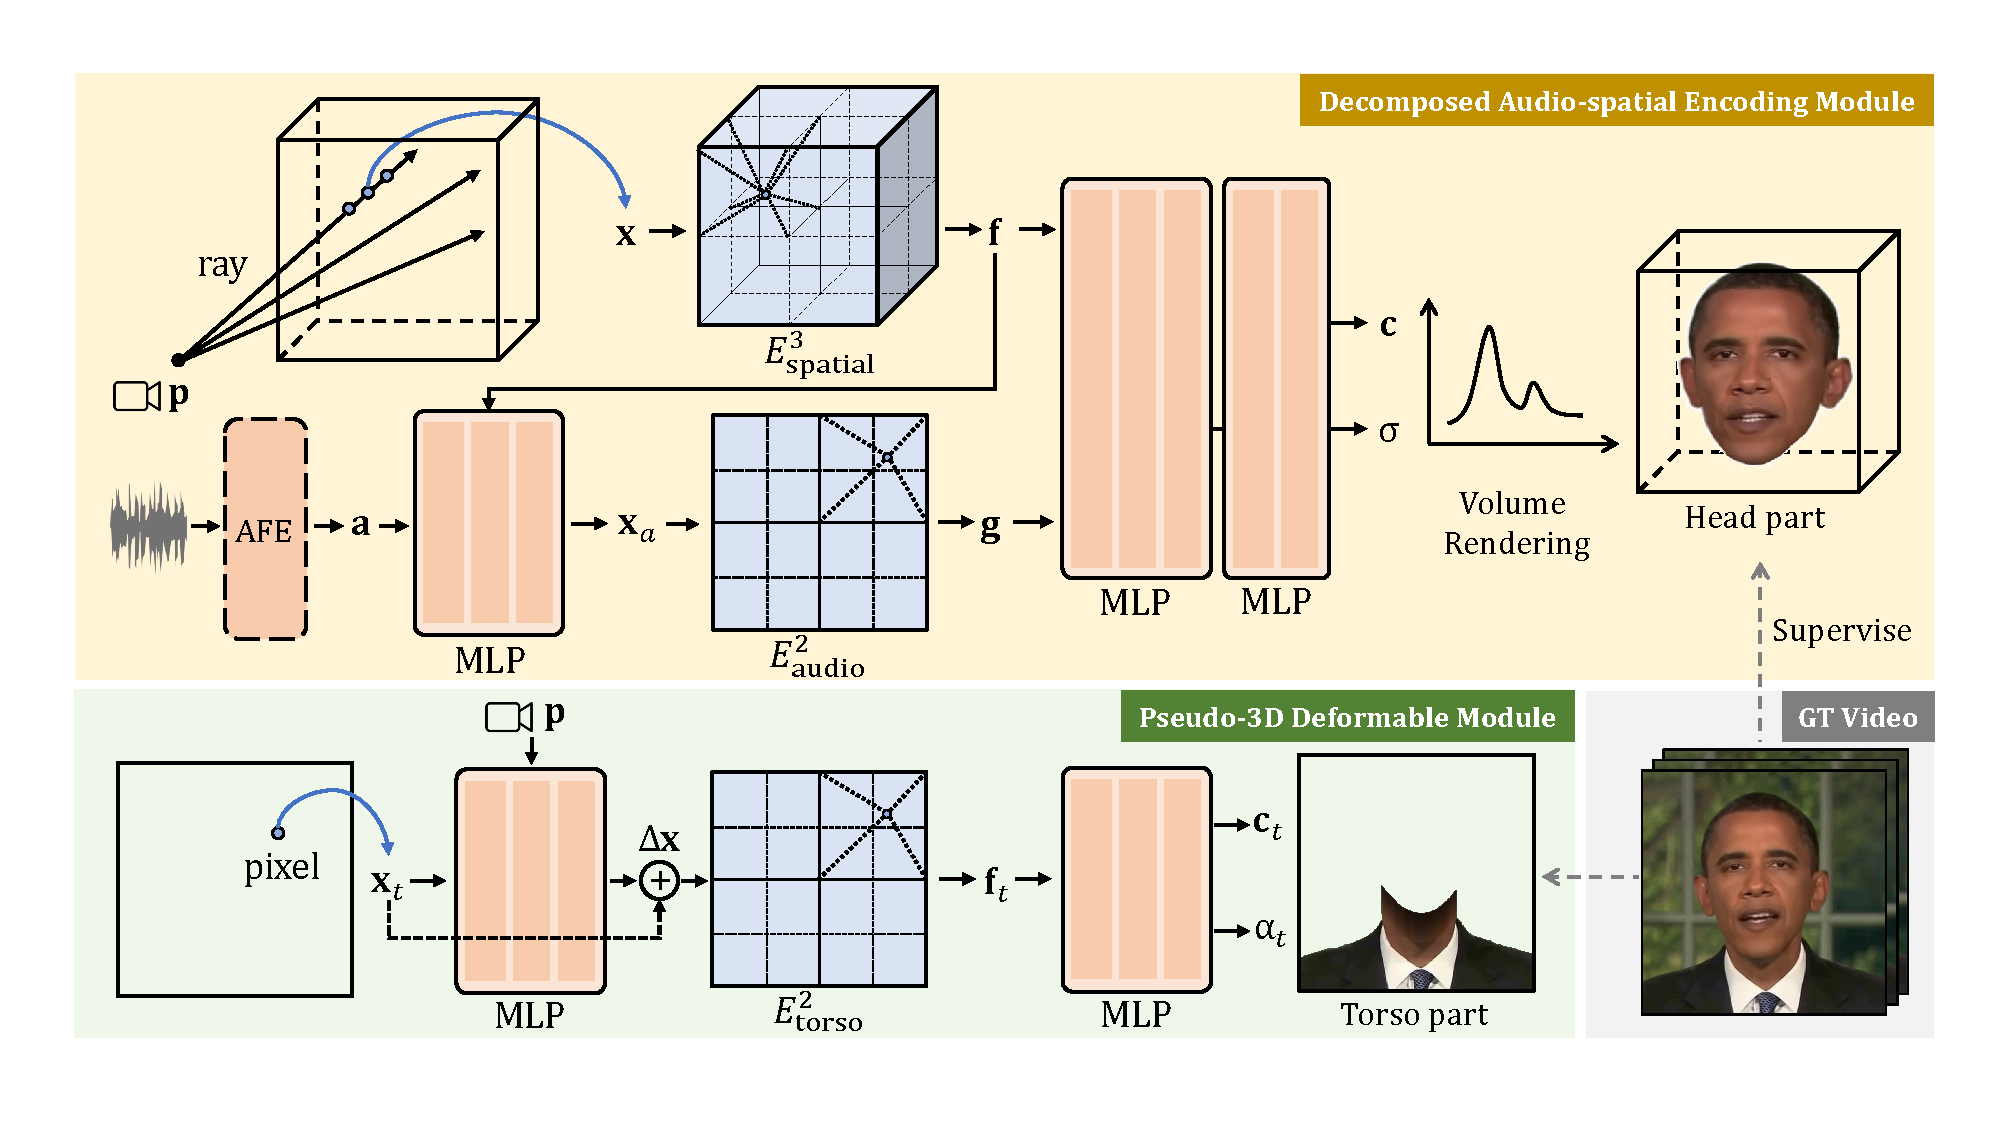
\includegraphics[width=0.8\textwidth]{figures/figure_chap_2/radnerf.pdf}
    \caption{Rad-NeRF Architecture}
    \label{fig:Rad-NeRF}
\end{figure} 

In decomposed audio-spatial encoding module, audio feature encoded from audio encoder models such as wav2vec2 or deepspeech, \cite{hjortnaes:2020, baevski2020wav2vec} and spatial features $\mathbf{f}$ encoded from 3D grid encoder $E^3_\text{spatial}$ are concatenated and fed into a fully-connected MLP to obtain the audio-spatial encoding $\mathbf{e}$.
Instead of utilizing a single, high-dimensional audio-spatial grid encoder represented as $\mathbf{g} = E^{3+D} (\mathbf{x}, \mathbf{x}a)$, the approach is restructured to employ two separate grid encoders with lower dimensions. These encoders are designated to process audio and spatial coordinates independently, with spatial features encoded as $\mathbf{f} = E^3\text{spatial} (\mathbf{x})$ and audio features as $\mathbf{g} = E^D_\text{audio} (\mathbf{x}_a)$. This modification significantly reduces the interpolation cost from $2^{3 + D}$ to a more manageable $2^3 + 2^D$ for $D \ge 1$. After the encoding process, the spatial and audio features, $\mathbf{f}$ and $\mathbf{g}$ respectively, are concatenated, facilitating subsequent interpolation steps. This strategy effectively simplifies the computational demands while preserving the detailed representation of audio-spatial data within the Neural Radiance Field framework.

% Citation 추가